\documentclass[12pt]{article}
\usepackage[english]{babel}
\usepackage[utf8x]{inputenc}
\usepackage{amsmath}
\usepackage{graphicx}
\usepackage[colorinlistoftodos]{todonotes}
\usepackage{pifont}
\usepackage{subfigure}% Support for small, `sub' figures and tables
\usepackage{float} 
\usepackage{array}
%\usepackage{url}
\usepackage[hyphens]{url} %break url
%\usepackage{xurl}
\usepackage{enumitem}
%\usepackage{biblatex}
\newcommand\tab[1][0.6cm]{\hspace*{#1}}
\usepackage{changepage}
\usepackage[nottoc]{tocbibind}



\usepackage{listings} % code listing
\usepackage{color}

\definecolor{dkgreen}{rgb}{0,0.6,0}
\definecolor{gray}{rgb}{0.5,0.5,0.5}
\definecolor{mauve}{rgb}{0.58,0,0.82}

\lstset{frame=tb,
    language=Java,
    aboveskip=3mm,
    belowskip=3mm,
    showstringspaces=false,
    columns=flexible,
    basicstyle={\scriptsize\ttfamily},
    numbers=none,
    numberstyle=\tiny\color{gray},
    keywordstyle=\color{blue},
    commentstyle=\color{dkgreen},
    stringstyle=\color{mauve},
    breaklines=true,
    breakatwhitespace=true,
    tabsize=3
}


\usepackage{csquotes}


\begin{document}
    
    \begin{titlepage}
        
        \newcommand{\HRule}{\rule{\linewidth}{0.5mm}} % Defines a new command for the horizontal lines, change thickness here
        
        \center % Center everything on the page
        
        %----------------------------------------------------------------------------------------
        %    HEADING SECTIONS
        %----------------------------------------------------------------------------------------
        
        \textsc{\large Central Washington University}\\[1.5cm] % Name of your university/college
        \textsc{\Large Advance Algorithm}\\[0.5cm] % Major heading such as course name
        \textsc{\large Winter 2020}\\[0.5cm] % Minor heading such as course title
        
        %----------------------------------------------------------------------------------------
        %    TITLE SECTION
        %----------------------------------------------------------------------------------------
        
        \HRule \\[0.5cm]
        { \LARGE \bfseries Project 1: k-Nearest Neighbor Search}\\[0.2cm] % Title of your document
        \HRule \\[0.5cm]
        
        %----------------------------------------------------------------------------------------
        %    AUTHOR SECTION
        %----------------------------------------------------------------------------------------
        
        %\begin{minipage}{0.5\textwidth}
        %    \begin{flushleft} \large
                \emph{Student:}
                %\begin{itemize}
                    \textsc {\large Tin Tan Nguyen} \\			
                 \emph{Email:}   ntin\textsc{@cwu.edu}\\
                %\end{itemize}
        %    \end{flushleft}
        %\end{minipage}
        ~
        %\begin{minipage}{0.45\textwidth}
        %    \begin{flushright} \large
        %        \emph{Professor:} \\
        %        Dr. Szilárd \textsc{VAJDA}\\ % Supervisor's Name
        %        Szilard.Vajda@cwu.edu
        %    \end{flushright}
        %\end{minipage}\\[0.5cm]
        
        % If you don't want a supervisor, uncomment the two lines below and remove the section above
        %\Large \emph{Author:}\\
        %John \textsc{Smith}\\[3cm] % Your name
        
        %----------------------------------------------------------------------------------------
        %    DATE SECTION
        %----------------------------------------------------------------------------------------
        \vspace{2cm}
        {\large \today}\\ % Date, change the \today to a set date if you want to be precise
        
        %----------------------------------------------------------------------------------------
        %    LOGO SECTION
        %----------------------------------------------------------------------------------------
        
        
\includegraphics[width=8cm]{CWU-Logo.png}\\[.5cm] % Include a department/university logo - this will require the graphicx package
        
        %----------------------------------------------------------------------------------------
        
        \vfill % Fill the rest of the page with whitespace
        
    \end{titlepage}
   
    
    \section{\large Time Complexity Analysis - Increasing N}
    \tab This section will discuss run time of k-nearest neighbor search using Python - scipy.spatial.kdtree package when increasing numbers of nearest neighbor.
    \begin{itemize}
    \item \textbf{Increasing N number of nearest neighbors:} 
    \begin{figure}[H]
    	\centering
    	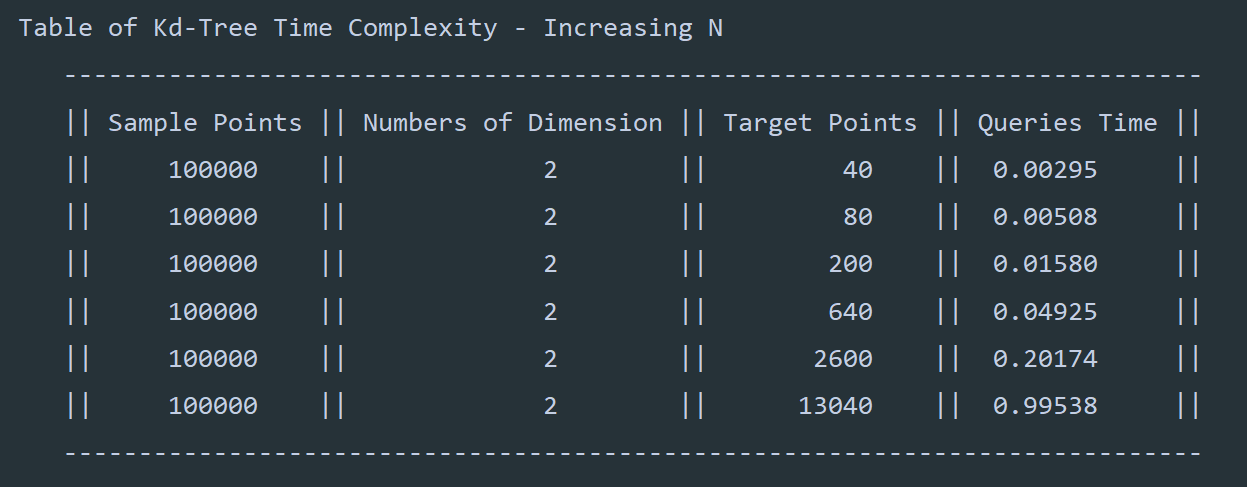
\includegraphics[width=14cm]{k-nearest-N-increase.png}
    	\caption{Time complexity when increasing N} 
    	\label{fig:1}
    \end{figure}
    \item \textbf{Time vs N-increasing Plot:}
    \begin{figure}[H]
    	\centering
    	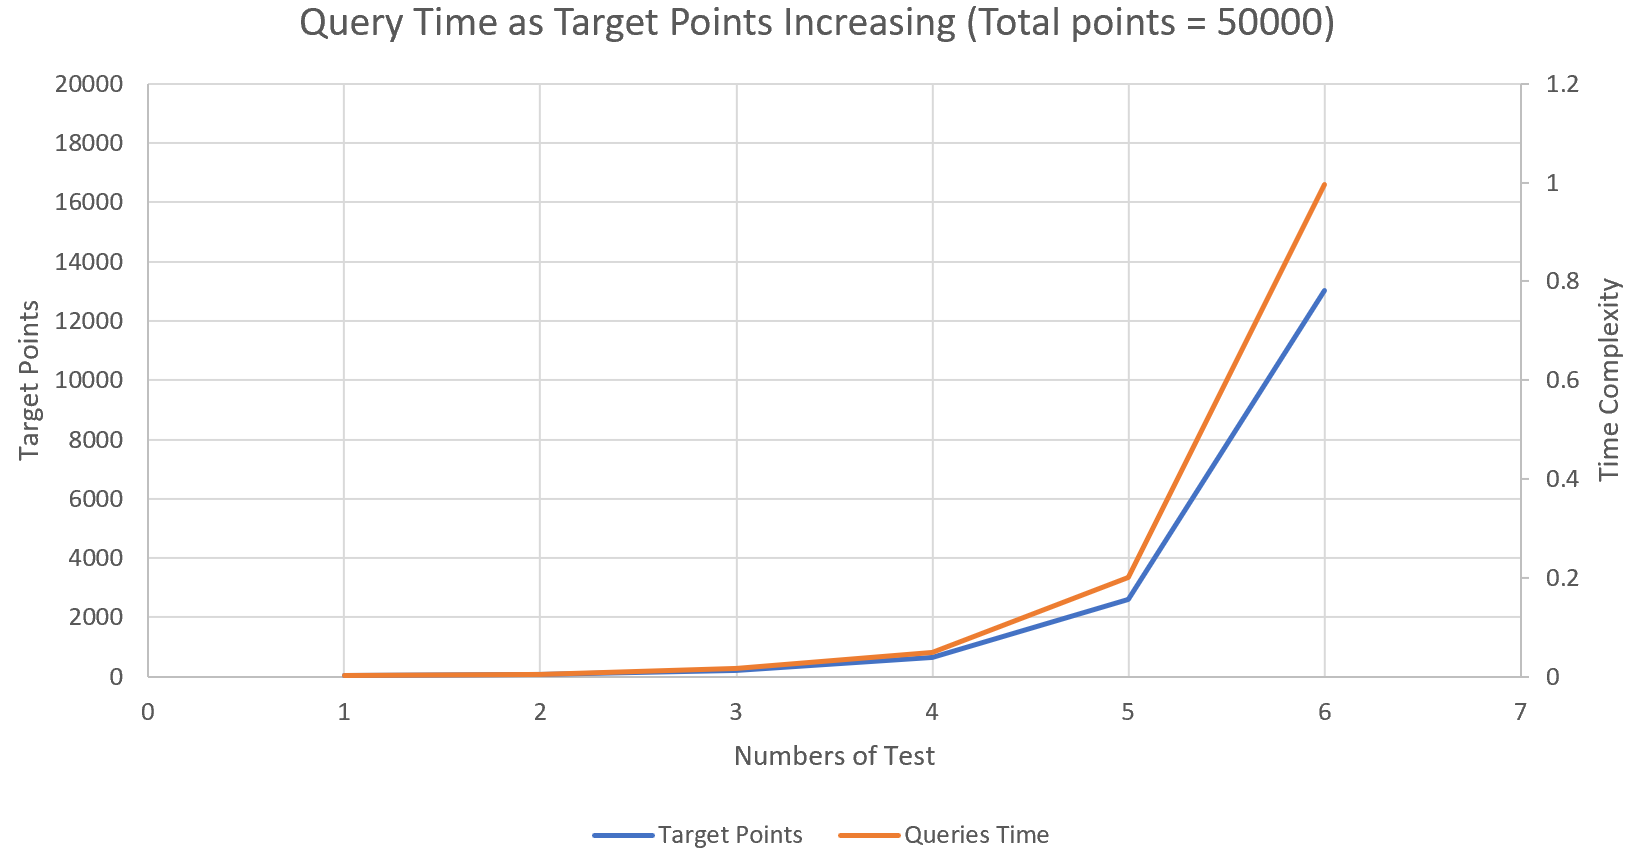
\includegraphics[width=13cm]{excel-N.PNG}
    	\caption{Time complexity as N increasing} 
    	\label{fig:2}
    	
    \end{figure}
    \end{itemize}
    \tab The relationship between run-time and N is almost linear by looking at the chart above (Time-complexity $<=$ TotalPoints)
 	\section{\large Time Complexity Analysis - Increasing D}
 	\tab This section will discuss run time of k-nearest neighbor search using Python - scipy.spatial.kdtree package when increasing dimension of nearest neighbor.
 	\begin{itemize}
    \item \textbf{Increasing number of dimensions (N = 5):} 
    \begin{figure}[H]
    	\centering
    	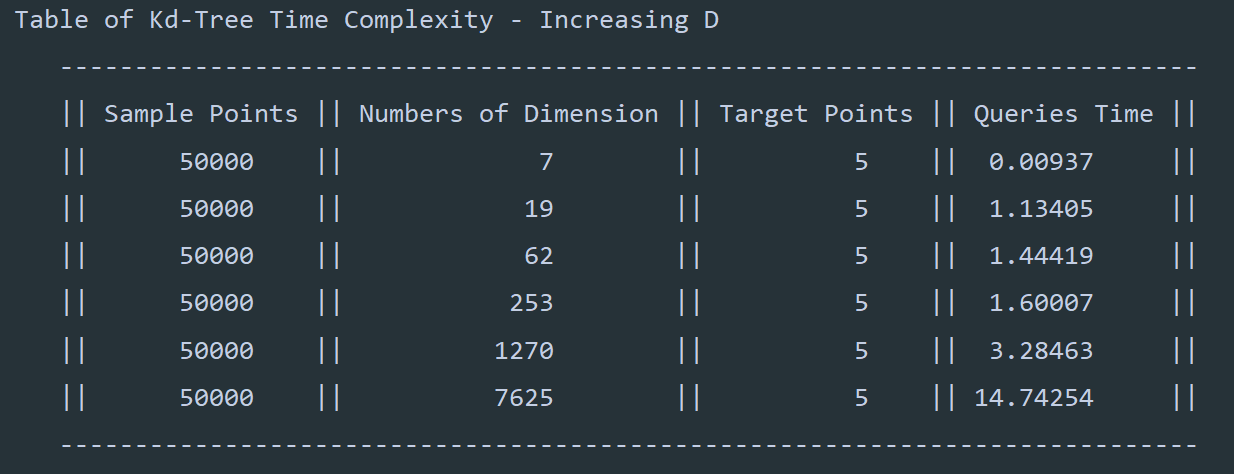
\includegraphics[width=14cm]{k-nearest-D-increase.png}
    	\caption{Time complexity when increasing D} 
    	\label{fig:3}
    \end{figure}
    \item \textbf{Time vs D-increasing Plot (NN = 5, Total Points = 50000):}
    \begin{figure}[H]
    	\centering
    	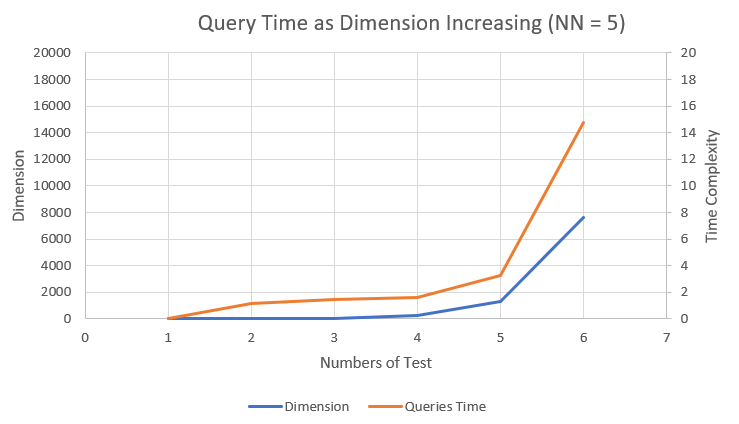
\includegraphics[width=14cm]{excel-D.PNG}
    	\caption{Time complexity as D increasing} 
    	\label{fig:4}
    \end{figure}
    \end{itemize}
    \tab The relationship between run-time and D is not a linear relationship by looking at the chart above (Time-complexity $>=$ TotalPoints and similar to log(TotalPoints)* TotalPoints.


	\section{\large Conclusion}
	\tab Time complexity of k-nearest neighbor algorithm is n times based on this project when increasing the NN numbers and about lg(n)n when increasing the dimension of NN. 
	\section{\large Python Code}
	\begin{figure}[H]
    	\centering
    	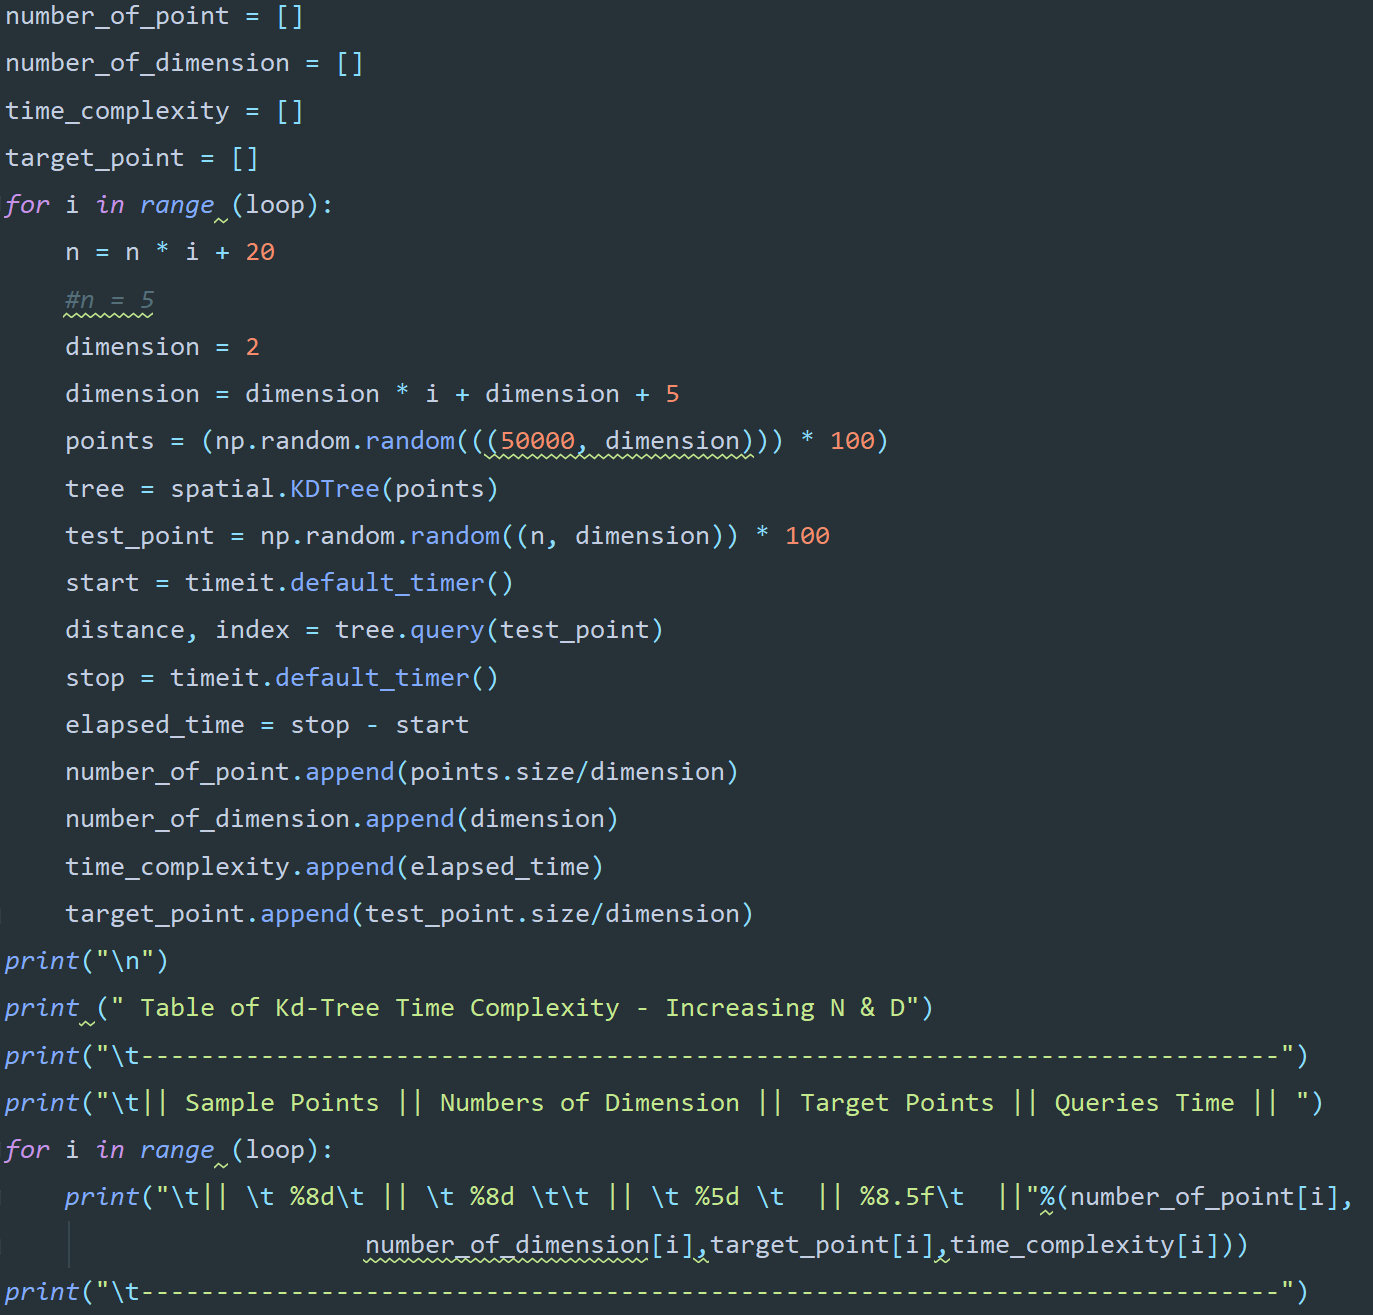
\includegraphics[width=14cm]{PythonCode.PNG}
    	\caption{Python Source Code} 
    	\label{fig:5}
    \end{figure}
    


\end{document}